% --- DOCUMENT DEFINITION ---
% we use article class because we want to fully customize the page and don't use a cv template
\documentclass[10pt,A4]{article}	

% --- ENCODING ---
% we use utf8 since we want to build from any machine
\usepackage[utf8]{inputenc}		

% --- LOGIC ---
% provides \isempty test
\usepackage{xstring, xifthen}

% --- FONT BASICS ---
%\usepackage[defaultsans]{droidsans}
%\usepackage[default]{comfortaa}
%\usepackage{cmbright}
\usepackage[default]{raleway}
%\usepackage{fetamont}
%\usepackage[default]{gillius}
%\usepackage[light,math]{iwona}
%\usepackage[thin]{roboto} 

% set font default
\renewcommand*\familydefault{\sfdefault} 	
\usepackage[T1]{fontenc}

% more font size definitions
\usepackage{moresize}

% --- FONT AWESOME ICONS ---
% include the fontawesome icon set
\usepackage{fontawesome}

% use to vertically center content
% credits to: http://tex.stackexchange.com/questions/7219/how-to-vertically-center-two-images-next-to-each-other
\newcommand{\vcenteredinclude}[1]{\begingroup
\setbox0=\hbox{\includegraphics{#1}}%
\parbox{\wd0}{\box0}\endgroup}

% use to vertically center content
% credits to: http://tex.stackexchange.com/questions/7219/how-to-vertically-center-two-images-next-to-each-other
\newcommand*{\vcenteredhbox}[1]{\begingroup
\setbox0=\hbox{#1}\parbox{\wd0}{\box0}\endgroup}

% icon shortcut
\newcommand{\icon}[3] { 							
	\makebox(#2, #2){\textcolor{maincol}{\csname fa#1\endcsname}}
}	

% icon with text shortcut
\newcommand{\icontext}[4]{ 						
	\vcenteredhbox{\icon{#1}{#2}{#3}}  \hspace{2pt}  \parbox{0.9\mpwidth}{\textcolor{#4}{#3}}
}

% icon with website url
\newcommand{\iconhref}[5]{ 						
    \vcenteredhbox{\icon{#1}{#2}{#5}}  \hspace{2pt} \href{#4}{\textcolor{#5}{#3}}
}

% icon with email link
\newcommand{\iconemail}[5]{ 						
    \vcenteredhbox{\icon{#1}{#2}{#5}}  \hspace{2pt} \href{mailto:#4}{\textcolor{#5}{#3}}
}

% --- PAGE LAYOUT  DEFINITIONS ---
% page outer frames (debug-only)
% \usepackage{showframe}		

% we use paracol to display breakable two columns
\usepackage{paracol}

% define page styles using geometry
\usepackage[a4paper]{geometry}

% remove all possible margins
\geometry{top=1cm, bottom=1cm, left=1cm, right=1cm}

\usepackage{fancyhdr}
\pagestyle{empty}

% space between header and content
% \setlength{\headheight}{0pt}

% indentation is zero
\setlength{\parindent}{0mm}

% TABLE /ARRAY DEFINITIONS
% extended aligning of tabular cells
\usepackage{array}

% custom column right-align with fixed width
% use like p{size} but via x{size}
\newcolumntype{x}[1]{%
>{\raggedleft\hspace{0pt}}p{#1}}%

% --- GRAPHICS DEFINITIONS ---
% for header image
\usepackage{graphicx}

% use this for floating figures
% \usepackage{wrapfig}
% \usepackage{float}
% \floatstyle{boxed} 
% \restylefloat{figure}

%for drawing graphics		
\usepackage{tikz}				
\usetikzlibrary{shapes, backgrounds,mindmap, trees}

% --- COLOR DEFINITIONS ---
\usepackage{transparent}
\usepackage{color}

% primary color
%\definecolor{maincol}{RGB}{ 0, 128, 255 }
\definecolor{maincol}{RGB}{ 48, 95, 118 }

% accent color, secondary
% \definecolor{accentcol}{RGB}{ 250, 150, 10 }

% dark color
\definecolor{darkcol}{RGB}{ 70, 70, 70 }

% light color
\definecolor{lightcol}{RGB}{245,245,245}


% Package for links, must be the last package used
\usepackage[hidelinks]{hyperref}

% returns minipage width minus two times \fboxsep
% to keep padding included in width calculations
% can also be used for other boxes / environments
\newcommand{\mpwidth}{\linewidth-\fboxsep-\fboxsep}
	

% --- CV COMMANDS ---
% --- CV LIST ---
% renders a standard latex list but abstracts away the environment definition (begin/end)
\newcommand{\cvlist}[1] {
	\begin{itemize}{#1}\end{itemize}
}

% --- CV TEXT ---
% base class to wrap any text based stuff here. Renders like a paragraph.
% Allows complex commands to be passed, too.
% param 1: *any
\newcommand{\cvtext}[1] {
	\begin{tabular*}{1\mpwidth}{p{0.98\mpwidth}}
		\parbox{1\mpwidth}{#1}
	\end{tabular*}
}

% --- CV SECTION ---
% Renders a a CV section headline with a nice underline in main color.
% param 1: section title
\newcommand{\cvsection}[1] {
	\vspace{14pt}
	\cvtext{
		\textbf{\LARGE{\textcolor{darkcol}{\uppercase{#1}}}}\\[-4pt]
		\textcolor{maincol}{ \rule{0.1\textwidth}{2pt} } \\
	}
}

% --- META SKILL ---
% Renders a progress-bar to indicate a certain skill in percent.
% param 1: name of the skill / tech / etc.
% param 2: level (for example in years)
% param 3: percent, values range from 0 to 1
\newcommand{\cvskill}[3] {
	\begin{tabular*}{1\mpwidth}{p{0.72\mpwidth}  r}
 		\textcolor{black}{\textbf{#1}} & \textcolor{maincol}{#2}\\
	\end{tabular*}%
	
	\hspace{4pt}
	\begin{tikzpicture}[scale=1,rounded corners=2pt,very thin]
		\fill [lightcol] (0,0) rectangle (1\mpwidth, 0.15);
		\fill [maincol] (0,0) rectangle (#3\mpwidth, 0.15);
  	\end{tikzpicture}%
}

% --- CV EVENT ---
% Renders a table and a paragraph (cvtext) wrapped in a parbox (to ensure minimum content
% is glued together when a pagebreak appears).
% Additional Information can be passed in text or list form (or other environments).
% the work you did
% param 1: time-frame i.e. Sep 14 - Jan 15 etc.
% param 2:	 event name (job position etc.)
% param 3: Customer, Employer, Industry
% param 4: Short description
% param 5: work done (optional)
% param 6: technologies include (optional)
% param 7: achievements (optional)
\newcommand{\cvevent}[7] {
	
	% we wrap this part in a parbox, so title and description are not separated on a pagebreak
	% if you need more control on page breaks, remove the parbox
	\parbox{\mpwidth}{
		\begin{tabular*}{1\mpwidth}{p{0.72\mpwidth}  r}
	 		\textcolor{black}{\textbf{#2}} & \colorbox{maincol}{\makebox[0.25\mpwidth]{\textcolor{white}{#1}}} \\
			\textcolor{maincol}{\textbf{#3}} & \\
		\end{tabular*}\\[8pt]
	
		\ifthenelse{\isempty{#4}}{}{
			\cvtext{#4}\\
		}
	}

	\ifthenelse{\isempty{#5}}{}{
		\vspace{9pt}
		{#5}
	}

	\ifthenelse{\isempty{#6}}{}{
		\vspace{9pt}
		\cvtext{\textbf{Technologies:}}\\
		{#6}
	}

	\ifthenelse{\isempty{#7}}{}{
		\vspace{9pt}
		\cvtext{\textbf{}}\\
		{#7}
	}
	\vspace{14pt}
}

% --- CV META EVENT ---
% Renders a CV event on the sidebar
% param 1: title
% param 2: subtitle (optional)
% param 3: customer, employer, etc,. (optional)
% param 4: info text (optional)
\newcommand{\cvmetaevent}[4] {
	\textcolor{maincol} {\cvtext{\textbf{\begin{flushleft}#1\end{flushleft}}}}

	\ifthenelse{\isempty{#2}}{}{
	\textcolor{darkcol} {\cvtext{\textbf{#2}} }
	}

	\ifthenelse{\isempty{#3}}{}{
		\cvtext{{ \textcolor{darkcol} {#3} }}\\
	}

	\cvtext{#4}\\[14pt]
}

% --- QR CODE ---
% Renders a qrcode image (centered, relative to the parentwidth)
% param 1: percent width, from 0 to 1
\newcommand{\cvqrcode}[1] {
	\begin{center}
		
\includegraphics[width={#1}\mpwidth]{qrcode}
	\end{center}
}

% --- DOCUMENT CONTENT ---
\begin{document}
\columnratio{0.31}
\setlength{\columnsep}{2.2em}
\setlength{\columnseprule}{4pt}
\colseprulecolor{lightcol}
\begin{paracol}{2}
\begin{leftcolumn}

% --- META IMAGE ---
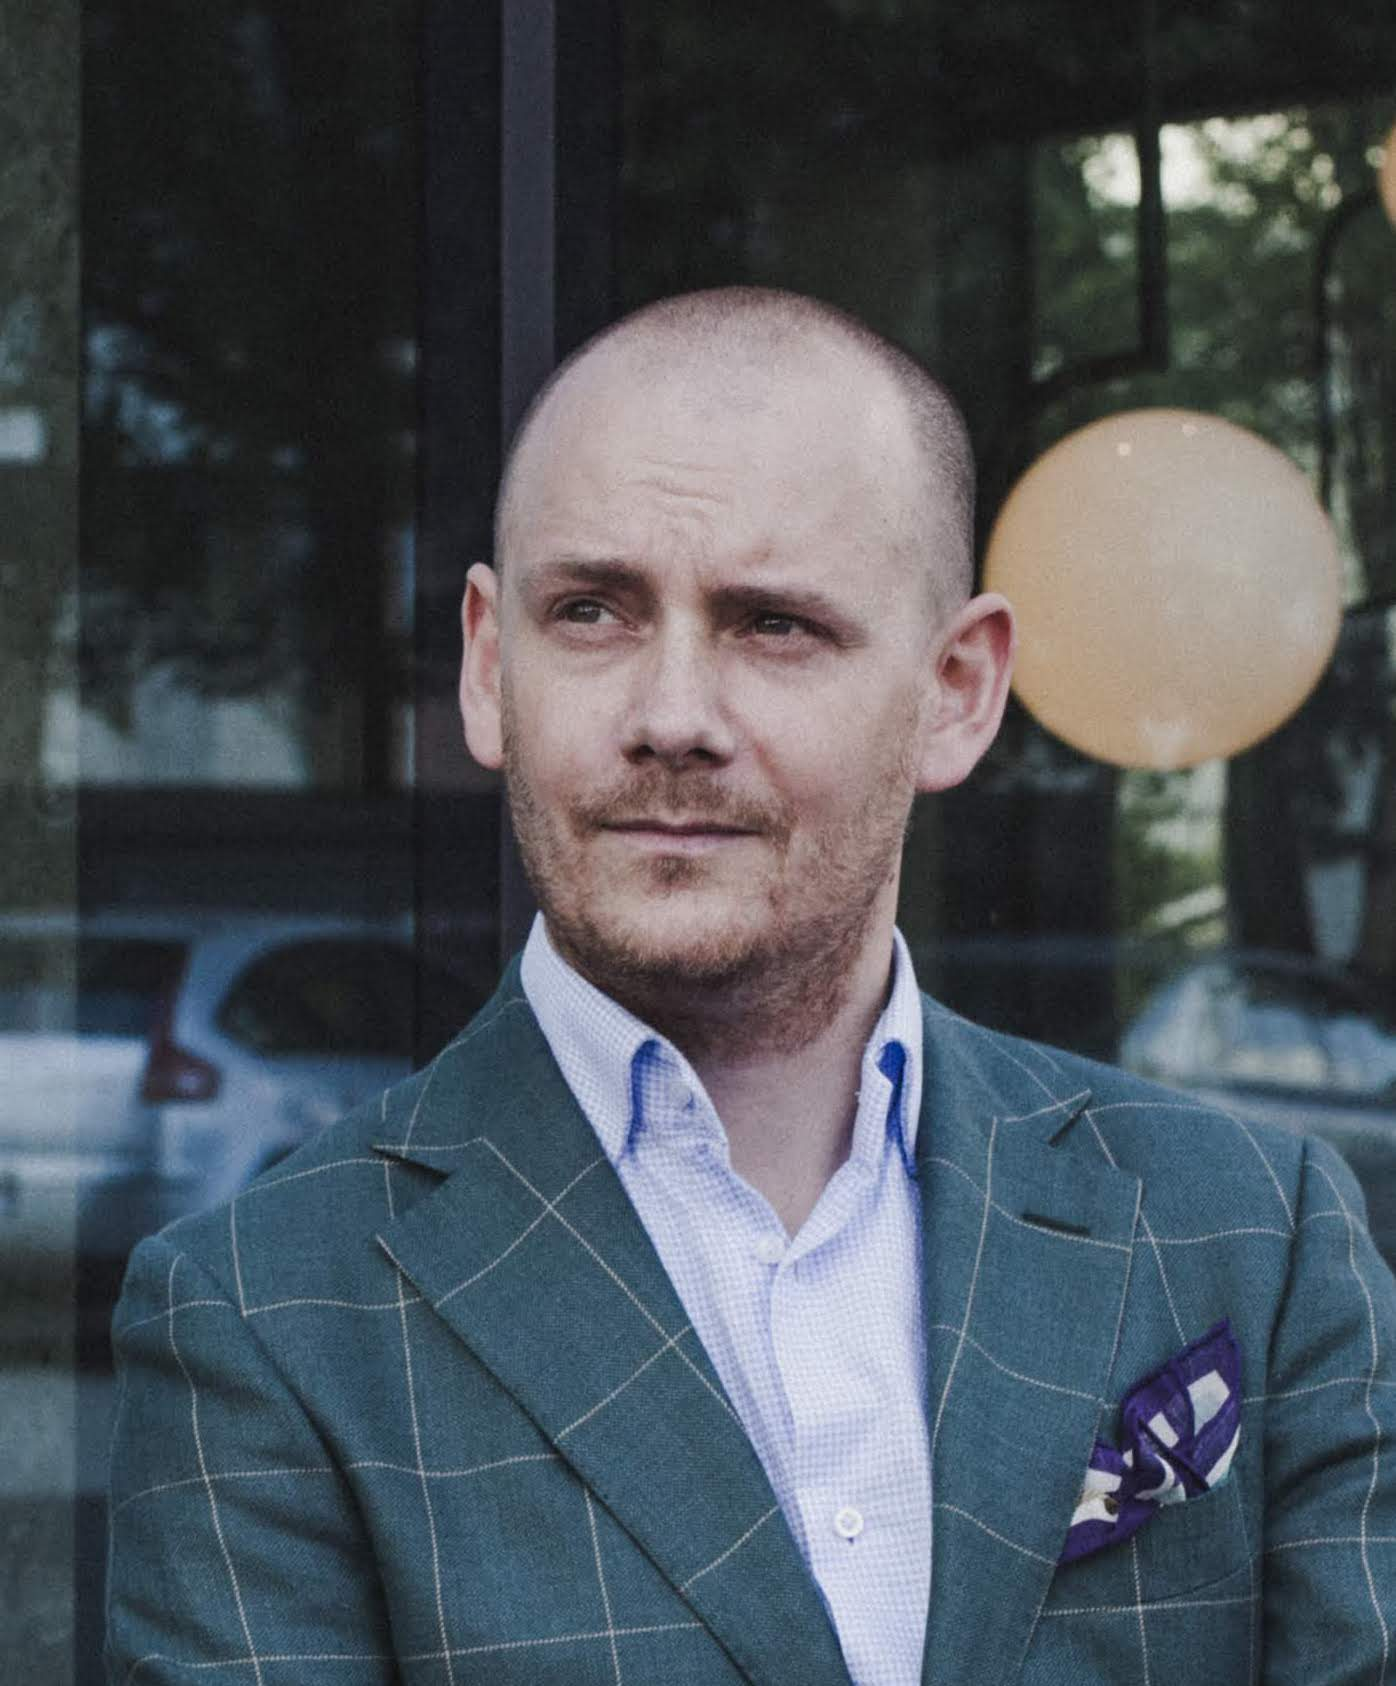
\includegraphics[width=\linewidth]{andrzejolender.jpg}	%trimming relative to image size

% --- META SKILLS ---
\cvsection{SKILLS}

\cvskill{Linux} {20 years} {0.9} \\[-2pt]

\cvskill{Kubernetes} {5 years} {0.8} \\[-2pt]

\cvskill{LGTM Stack} {5 years} {0.7} \\[-2pt]

\cvskill{Ansible} {4 year} {0.7} \\[-2pt]

\cvskill{CI/CD GitLab/GitHub} {4 years} {0.7} \\[-2pt]

\cvskill{Terraform} {3 years} {0.7} \\[-2pt]

\cvsection{CERTIFICATES}
\cvtext{Certified Kubernetes Administrator}{black}\\[6pt]
\vfill\null

\cvsection{CONTACT}

\icontext{Phone}{12}{+48 731 017 202}{black}\\[6pt]
\iconemail{Envelope}{12}{andrzej@olender.io}{andrzej@olender.io}{black}\\[6pt]
\iconhref{Globe}{12}{olender.io}{https://olender.io}{black}\\[6pt]

\vfill\null
\cvqrcode{0.7}


% --- EDUCATION ---
\newpage
\cvsection{EDUCATION}

\cvmetaevent
{2003 - 2005}
{Technical School}
{Post-Secondary Vocational School}
{IT Technician. Thesis defense: Security of Servers Based on the Linux System}

\cvmetaevent
{1997 - 2002}
{Technical School}
{School Complex No. 2, Tychy}
{Automation Technician. Specialization: Control and Measurement Apparatus and Mechanical Industrial Automation}

% --- HOBBY ---
\cvsection{HOBBY}

\cvmetaevent
{}
{}
{}
{Home automation (Home Assistant, ESP, Zigbee, etc.). Long-distance running, photography (formerly professional), manual craftsmanship (patination of classic footwear, 2nd place at the World Championships - London 2019) }
\vfill

\mbox{} % hotfix to place qrcode on the bottom when there are not other elements
\vfill
\end{leftcolumn}
\begin{rightcolumn}

% --- TITLE  HEADER ---
\fcolorbox{white}{white}{\begin{minipage}[c][3.5cm][c]{1\mpwidth}
	\begin {center}
		\HUGE{ \textbf{ \textcolor{darkcol}{ \uppercase{ Andrzej Olender } } } } \\[-24pt]
		\textcolor{darkcol}{ \rule{0.1\textwidth}{1.25pt} } \\[4pt]
		\large{ \textcolor{darkcol} {Happy Engineer} }
	\end {center}
\end{minipage}} \\[14pt]
\vspace{-12pt}

% --- PROFILE ---
\cvsection{ABOUT ME}

\cvtext{I have been active in the Linux community since 1998, and I am a strong advocate of Open Source and technology in general.\\

I specialize in automations, from those that bring benefits in private life (Smart Home) to producing and delivering software in business. I am a fervent fan of "Everything as Code".\\

Nearly 20 years of professional experience allows me to now look at many potential problems from an unconventional perspective.\\

I am able to work under stress, communicate well with teams of people, and am a team player.\\
}


% --- WORK EXPERIENCE ---
\cvsection{WORK EXPERIENCE}
\cvevent
    {Nov 21 - Present}
    {Site Reliability Engineer (SRE)}
    {eSky.pl S.A}
    {Development and maintenance of hybrid Google Cloud/On-prem infrastructure}
    {\cvlist{
        \item Automation of processes, planning of SLI/SLO/SLA services.
        \item Solving current problems, migration of onprem services to the GCP
        \item Infrastructure development
        \item Working in the SCRUM methodology
    }}
    {\cvlist {
        \item Google Cloud, Terraform, Ansible
        \item Kubernetes, Consul
        \item PostgreSQL, MongoDB, Redis, Kafka
        \item ArgoCD, Spinnaker, Jenkins
        \item Confluence, Bitbucket
        \item Prometheus, Grafana, ELK Stack
        \vfill
    }}
\vfill\null
\cvevent
    {Feb 21 - Nov 21}
    {DevOps Engineer}
    {Saint Gobain Sekurit}
    {Development and maintenance of infrastructure in 30 on-premise locations worldwide}
    {\cvlist{
        \item Writing GitLab CI/CD pipelines
        \item Process automation
        \item Implementation of the first Kubernetes clusters in the organization
        \item Collaborating with developers on migrating applications to k8s
        \item Writing Yaml/Kustomize/Helm manifests
        \item Implementing a GitOps-compliant policy
        \item Working in the SCRUM methodology
    }}
    {\cvlist {
        \item Kubernetes, Docker
        \item PostgreSQL, MongoDB
        \item GitLab, Sentry
        \item Apache Kafka, MQTT
        \item Zabbix, Prometheus, Grafana
        \vfill
    }}
\vfill\null
\cvevent
    {Aug 17 - Jan 21}
    {Senior Software Deployment Specialist}
    {Yakudo Plus}
    {Software deployment in the manufacturing industry, close cooperation with the software development department}
    {\cvlist{
        \item Implementing industry-supporting software
        \item Conducting training for business partners
        \item Preparing pre-implementation analyses
        \item Developing deployment documentation
        \item Providing assistance to end customers
        \item Working in the SCRUM methodology
    }}
    {\cvlist {
        \item MySQL, MSSQL, PostgreSQL
        \item GitLab
        \item Docker
        \item Linux Embedded
    }}
\vfill\null
\cvevent
    {Oct 02 - Aug 17}
    {Senior Technical Specialist}
    {Yakudo Plus}
    {Service of electronic labeling devices. Implementing devices along with software for marking goods in industrial production (EAN13, EAN128, QR Code)}
    {\cvlist{
        \item Support service for labeling devices along with software
        \item Customer assistance - Help Desk
        \item Creating service documentation
        \item Conducting training for service partners
    }}
    {\cvlist {
        \item .NET
        \item MySQL
        \item Linux Embedded 
    }}
	

	
% hotfixes to create fake-space to ensure the whole height is used
\mbox{}
\vfill
\mbox{}
\vfill
\mbox{}
\vfill
\mbox{}
\end{rightcolumn}
\end{paracol}
\vfill\null
\footref{
% Wyrażam zgodę na przetwarzanie moich danych osobowych dla potrzeb niezbędnych do realizacji procesu rekrutacji (zgodnie z ustawą z dnia 10 maja 2018 roku o ochronie danych osobowych (Dz. Ustaw z 2018, poz. 1000) oraz zgodnie z Rozporządzeniem Parlamentu Europejskiego i Rady (UE) 2016/679 z dnia 27 kwietnia 2016 r. w sprawie ochrony osób fizycznych w związku z przetwarzaniem danych osobowych i w sprawie swobodnego przepływu takich danych oraz uchylenia dyrektywy 95/46/WE (RODO)}
\end{document}
